\chapter{Théorie et Modélisation}
\label{chap:3-Theory}

\section{Dynamique du Système}

\paragraph{Le système de stabilisation de la barre rotative est un système dynamique non linéaire à un degré de liberté. Le système est composé d'une barre rotative montée sur un support fixe. La barre rotative est contrôlée par deux rotors qui peuvent appliquer un couple sur la barre pour la stabiliser.}

\paragraph{Le système est soumis à plusieurs forces et moments qui influent sur son mouvement. Les forces et moments les plus importants sont :}

\begin{enumerate}
	\item \textbf{Force de gravité :} La force de gravité agit sur la barre rotative et exerce un couple sur la barre.
	\item \textbf{Couple des rotors :} Les rotors peuvent appliquer un couple sur la barre pour la stabiliser.
	\item \textbf{Frottement :} Le frottement entre la barre rotative et le support fixe peut ralentir le mouvement de la barre.
\end{enumerate}

\begin{figure}[!htpb]
	\centering
	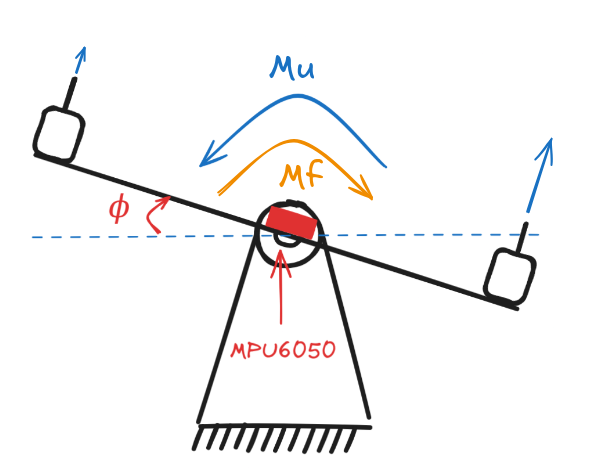
\includegraphics[width=0.6\linewidth]{Figures/moments.png}
	\caption{Moments de Force.}
\end{figure}

\paragraph{Le système est décrit par l'équation dynamique suivante :}

\begin{equation}
	J_\Delta * \frac{d^2\phi}{dt^2} = \sum M
\end{equation}

\subsubsection{Moments de Force :}
\begin{itemize}
	\item $M_f$: est le moment de force dû au frottement. $M_f = -f * \frac{d\phi}{dt}$.
	\item $M_g$: est le moment de force dû à la gravité (Si centre de masse coincide avec centre geometrique alors $M_g$ = 0).
	\item $M_{u}$: est le moment de force dû aux rotors. (Directement proportionnel à l'entrée $u$).
\end{itemize}

\begin{equation}
	J_\Delta * \frac{d^2\phi}{dt^2} = M_{u} - f * \frac{d\phi}{dt}
\end{equation}

\begin{itemize}
	\item $\phi$ est l'angle de la barre rotative par rapport à l'horizontale $0^\circ $.
	\item $J_\Delta$ est le moment d'inertie de la barre rotative.
	\item $L$ est la longueur de la barre rotative.
	\item $f$ est le coefficient de frottement.
\end{itemize}

\subsection{Commande simplifiée}

\paragraph{Pour simplifier la commande du système due à la symmétrie du système, on peut utiliser une commande sous forme scalaire. avec $F$ la force mediane des rotors.}
\paragraph*{}
\begin{figure}[!htpb]
	\centering
	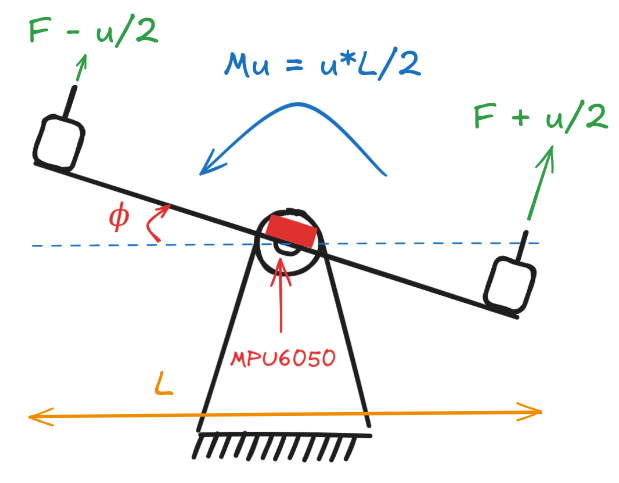
\includegraphics[width=0.8\linewidth]{Figures/Mu.png}
	\caption{Commande scalaire.}
\end{figure}

\begin{equation}
	M_u = M_{rotor1} + M_{rotor2}
\end{equation}

\begin{equation}
	M_u = \frac{L}{2} * ((F + \frac{u}{2}) - (F - \frac{u}{2}))
\end{equation}

\begin{equation}
	M_u = u * \frac{L}{2}
\end{equation}

\paragraph{L'equation dynamique du système devient :}
\begin{equation}
	J_\Delta * \frac{d^2\phi}{dt^2} + f * \frac{d\phi}{dt} = u * \frac{L}{2}
\end{equation}

\subsubsection{Limitation}

\paragraph{Le problème le plus pertinent dans cette approche de commande est le faite que les deux motors ne sont pas physiquement les mêmes, donc pour la même consigne les deux rotors ne vont pas tourner à la même vitesse.}


\subsection{Systeme en boucle ouverte}

\subsubsection{Equation dynamique}

\begin{equation}
	J_\Delta * \frac{d^2\phi}{dt^2} + f * \frac{d\phi}{dt} = u * \frac{L}{2}
\end{equation}

\subsubsection{Transformée de Laplace}

\begin{equation}
	J_\Delta * s^2 * \Phi(s) + f * s * \Phi(s) = U(s) * \frac{L}{2}
\end{equation}

\begin{equation}
	G(s) = \frac{\Phi(s)}{U(s) * \frac{L}{2}} = \frac{1}{J_\Delta * s^2 + f * s}
\end{equation}

\paragraph{Le système est du second ordre mais non standard car le terme constant est nul $\omega_n = 0$ avec deux poles réels:}

\begin{itemize}
	\item \textbf{Pole 1 :} $s_1 = 0$
	\item \textbf{Pole 2 :} $s_2 = -\frac{f}{J_\Delta}$
\end{itemize}

\subsubsection{Remarques}

\begin{itemize}
	\item $J_\Delta > 0$, $f > 0$, donc $s_2 < 0$. $s_2$ dans la region de stabilité.
	\item Par contre, $s_1$ est nul, donc le système est marginalement stable.
	\item Peut être stabilisé en ajoutant un PID.
	\begin{itemize}
		\item \textbf{P :} Pour rendre le système standard mais pas suffisant car il y aura un erreur statique.
		\item \textbf{I :} Pour éliminer l'erreur statique.
		\item \textbf{D :} Pour un meilleur amortissement.
	\end{itemize}
\end{itemize}


\subsubsection{Dynamique dyu système sous forme d'espace d'état}


\begin{equation}
	\frac{dx}{dt} = A * x + B * u
\end{equation}

\begin{equation}
	y = C * x
\end{equation}

\begin{equation}
	\begin{bmatrix}
		\frac{d\phi}{dt} \\
		\frac{d^2\phi}{dt^2}
	\end{bmatrix}
	=
	\begin{bmatrix}
		0 & 1 \\
		0 & -\frac{f}{J_\Delta}
	\end{bmatrix}
	\begin{bmatrix}
		\phi \\
		\frac{d\phi}{dt}
	\end{bmatrix}
	+
	\begin{bmatrix}
		0 \\
		\frac{L}{2J_\Delta}
	\end{bmatrix}
	u
\end{equation}

\begin{equation}
	y = \begin{bmatrix}
		1 & 0
	\end{bmatrix}
	\begin{bmatrix}
		\phi \\
		\frac{d\phi}{dt}
	\end{bmatrix}
\end{equation}

\subsubsection{Matrice de commandabilité :}

\begin{equation}
	A * B = \begin{bmatrix}
		0 & 1 \\
		0 & -\frac{f}{J_\Delta}
	\end{bmatrix}
	\begin{bmatrix}
		0 \\
		\frac{L}{2J_\Delta}
	\end{bmatrix}
	=
	\begin{bmatrix}
		\frac{L}{2J_\Delta} \\
		-\frac{fL}{2J_\Delta^2}
	\end{bmatrix}
\end{equation}

\begin{equation}
	M_c = \begin{bmatrix}
		B & A * B
	\end{bmatrix}
	= \begin{bmatrix}
		0 & \frac{L}{2J_\Delta} \\
		\frac{L}{2J_\Delta} & -\frac{fL}{2J_\Delta^2}
	\end{bmatrix}
	= \frac{L}{2J_\Delta}
	\begin{bmatrix}
		0 & 1 \\
		1 & -\frac{f}{J_\Delta}
	\end{bmatrix}
\end{equation}

\begin{equation}
	\text{rang}(M_c) = 2 \Rightarrow \text{commandable}
\end{equation}

\subsubsection{Matrice d'observabilité :}

\begin{equation}
	C * A = \begin{bmatrix}
		1 & 0
	\end{bmatrix}
	\begin{bmatrix}
		0 & 1 \\
		0 & -\frac{f}{J_\Delta}
	\end{bmatrix}
	= \begin{bmatrix}
		0 & 1
	\end{bmatrix}
\end{equation}

\begin{equation}
	M_o = \begin{bmatrix}
		C \\
		C * A
	\end{bmatrix}
	= \begin{bmatrix}
		1 & 0 \\
		0 & 1
	\end{bmatrix}
	= \begin{bmatrix}
		1 & 0 \\
		0 & 1
	\end{bmatrix}
\end{equation}

\begin{equation}
	\text{rang}(M_o) = 2 \Rightarrow \text{observable}
\end{equation}

\section{Correcteur PID}

\paragraph{D'apres les remarques précédentes, on peut utiliser un correcteur PID pour stabiliser le système.}

\begin{equation}
	u(t) = K_p e(t) + K_i \int_{0}^{t} e(\tau) \,d\tau + K_d \frac{de(t)}{dt}
\end{equation}

\begin{equation}
	C(s) = \frac{U(s)}{E(s)} = K_p + K_i * \frac{1}{s} + K_d * s
\end{equation}

\begin{equation}
	G(s) = \frac{1}{J_\Delta * s^2 + f * s}
\end{equation}

\begin{figure}[!htpb]
	\centering
	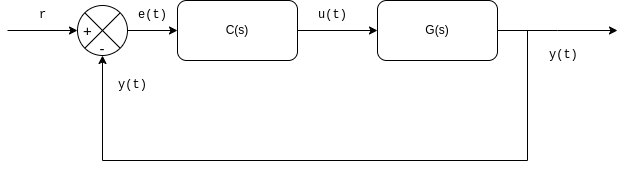
\includegraphics[width=\linewidth]{Figures/sys+correcteur.png}
	\caption{Correcteur PID.}
\end{figure}

\begin{equation}
	FTBO(s) = C(s) * G(s) = \frac{K_d * s^2 + K_p * s + Ki}{J_\Delta * s^3 + f * s^2}
\end{equation}

\begin{equation}
	FTBF(s) = \frac{C(s) * G(s)}{1 + C(s) * G(s)} = \frac{K_d * s^2 + K_p * s + Ki}{J_\Delta * s^3 + (f + K_d) * s^2 + K_p * s + Ki}
\end{equation}

\subsection{Stabilité}

\begin{equation}
	D(s) = J_\Delta * s^3 + (f + K_d) * s^2 + K_p * s + Ki
\end{equation}

Tous les coefficients de $D(s)$ doivent être positifs pour que le système soit stable (Pas suffisant mais nécessaire).

\begin{itemize}
	\item $J_\Delta > 0$, (toujours vrai).
	\item $f + K_d > 0$, 
	\item $K_p > 0$.
	\item $Ki > 0$.
\end{itemize}

\subsubsection{Critère de Routh-Hurwitz}

\begin{equation}
	\begin{array}{c|c c}
		s^3 & J_\Delta & K_p \\
		s^2 & f + K_d & Ki \\
		s^1 & \frac{K_p * (f + K_d) - J_\Delta * Ki}{f + K_d} & 0 \\
		s^0 & Ki & 0
	\end{array}
\end{equation}

\begin{itemize}
	\item $J_\Delta > 0$, (toujours vrai).
	\item $f + K_d > 0$, 
	\item $K_p * (f + K_d) > J_\Delta * Ki$.
	\item $Ki > 0$.
\end{itemize}

\newpage

\subsection{Conclusion}

\paragraph{Fonction de tranfert du système avec correcteur PID en boucle fermée :}

\begin{equation}
	H_{des}(s) = \frac{K_d * s^2 + K_p * s + Ki}{J_\Delta * s^3 + (f + K_d) * s^2 + K_p * s + Ki}
\end{equation}

\paragraph{Le système avec correcteur en boucle fermée est stable si les conditions suivantes sont vérifiées :}

\begin{itemize}
	\item $K_d > -f$.
	\item $K_p * (f + K_d) > J_\Delta * Ki$.
	\item $Ki > 0$.
	\item $K_p > 0$.
\end{itemize}


\section{Calcul de l'orientation}

\paragraph{Le capteur MPU6050 est un capteur d'inertie à six degrés de liberté qui combine un accéléromètre et un gyroscope pour mesurer l'orientation d'un objet dans l'espace tridimensionnel. L'accéléromètre mesure l'accélération linéaire de l'objet, tandis que le gyroscope mesure la vitesse angulaire de l'objet.}

\paragraph{Alors pour savoir l'orientation de l'objet, on doit envisager un algorithme pour calculer l'angle d'orientation.}

\subsubsection{Les Angles d'Euler}

\paragraph{Les angles d'Euler sont une méthode courante pour représenter l'orientation d'un objet dans l'espace tridimensionnel. Les angles d'Euler sont composés de trois angles : l'angle de roulis, l'angle de tangage et l'angle de lacet. Ces angles décrivent la rotation de l'objet autour de ses axes X, Y et Z respectivement d'un système de coordonnées fixe.}

\begin{enumerate}
	\item \textbf{Roulis (Roll) :} Rotation autour de l'axe X. $\theta$.
	\item \textbf{Tangage (Pitch) :} Rotation autour de l'axe Y. $\phi$.
	\item \textbf{Lacet (Yaw) :} Rotation autour de l'axe Z. $\psi$.
\end{enumerate}


\subsubsection{La matrice de rotation}

\begin{equation*}
	R_x = \begin{bmatrix}
		1 & 0 & 0 \\
		0 & \cos(\theta) & -\sin(\theta) \\
		0 & \sin(\theta) & \cos(\theta)
	\end{bmatrix}
\end{equation*}

\begin{equation*}
	R_y = \begin{bmatrix}
		\cos(\phi) & 0 & \sin(\phi) \\
		0 & 1 & 0 \\
		-\sin(\phi) & 0 & \cos(\phi)
	\end{bmatrix}
\end{equation*}

\begin{equation*}
	R_z = \begin{bmatrix}
		\cos(\psi) & -\sin(\psi) & 0 \\
		\sin(\psi) & \cos(\psi) & 0 \\
		0 & 0 & 1
	\end{bmatrix}
\end{equation*}

\begin{equation*}
	R_{xyz} = R_x(\theta) \times R_y(\phi) \times R_z(\psi)
\end{equation*}

\begin{equation*}
	R_{xyz} = \begin{bmatrix}
		\cos(\phi) \cos(\psi) & \cos(\phi) \sin(\psi) & -\sin(\phi) \\
		\sin(\theta) \sin(\phi) \cos(\psi) - \cos(\theta) \sin(\psi) & \sin(\theta) \sin(\phi) \sin(\psi) + \cos(\theta) \cos(\psi) & \sin(\theta) \cos(\phi) \\
		\cos(\theta) \sin(\phi) \cos(\psi) + \sin(\theta) \sin(\psi) & \cos(\theta) \sin(\phi) \sin(\psi) - \sin(\theta) \cos(\psi) & \cos(\theta) \cos(\phi)
	\end{bmatrix}
\end{equation*}

\paragraph{On définit la matrice R de rotation du capteur par rapport au repère fixe.}

\begin{equation}
	R = R_{xyz}
\end{equation}

\subsection{Accéléromètre}


\subsubsection{Modèle Mathématique}

\paragraph{L'accélération linéaire mesurée par l'accéléromètre est composée, l'accélération gravitationnelle et de l'accélération linéaire de l'objet, le biais de l'accéléromètre et le bruit de l'accéléromètre.}

\begin{equation}
	\vec{a} = \frac{\vec{dv}}{dt} - R * \vec{g} + b_a(t) + n_a(t)
\end{equation}

\begin{itemize}
	\item $\vec{a}$ est l'accélération linéaire mesurée par l'accéléromètre.
	\item $R$ est la matrice de rotation du capteur.
	\item $b_a(t)$ est le biais de l'accéléromètre.
	\item $n_a(t)$ est le bruit de l'accéléromètre.
\end{itemize}

\paragraph{L'accélération gravitationnelle est définie comme :}
\begin{equation*}
	g = 9.81 \, m/s^2
\end{equation*}

\begin{equation*}
	g = 1 gram\\
\end{equation*}

\paragraph*{Pour une plage de mesure de l'accéléromètre de $\pm 4g$ on a :}

\begin{equation*}
	g = \frac{2^{16}}{8grams} * 1gram = 8192\hspace*{.2cm}(raw\hspace*{.1cm}sensor)
\end{equation*}



\paragraph{Dans un premier temps on se pose au repos donc l'accélération linéaire est nulle aussi nous allons négliger le bruit et le biais de l'accéléromètre pour simplifier le modèle.}

\begin{equation*}
	\vec{a} = -R * \vec{g}
\end{equation*}

\paragraph{On deduit trois equations pour les trois axes de l'accéléromètre.}

\begin{align*}
	a_x &= g \sin(\phi) \\
	a_y &= -g \sin(\theta) \cos(\phi)\\
	a_z &= -g \cos(\theta) \cos(\phi)
\end{align*}

\paragraph{Pour ce projet notre bras posede un seul degré de liberté, donc nous allons utiliser l'angle de tangage pour déterminer la position du bras.}


\begin{equation}
	\hat{\phi}_{accelo}(n) = \arcsin\left(\frac{a_x(n)}{g}\right)
\end{equation}

\paragraph{Le problème de cette estimation de l'orientation est que l'accéléromètre est bruité et sensible aux vibrations. L'estimation de l'orientation à partir de l'accéléromètre est sujette à des erreurs et des dérives.}

\begin{figure}[!htpb]
	\centering
	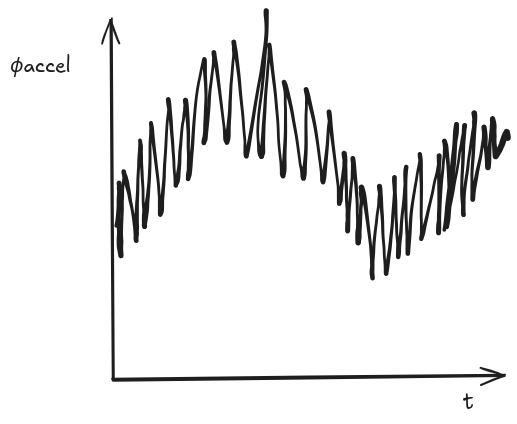
\includegraphics[width=0.7\linewidth]{Figures/accel-limits.png}
	\caption{Accéléromètre Limitation.}
\end{figure}

\paragraph{}
\subsection{Gyroscope}

\paragraph{L'intégrale de la rotation est une méthode simple pour estimer l'orientation d'un objet à partir des données d'un gyroscope. L'intégrale de la rotation consiste à intégrer les données du gyroscope pour estimer l'orientation de l'objet en temps réel.}

\subsubsection{Modèle Mathématique}

\paragraph{La vitesse angulaire mesurée par le gyroscope est composée de la vitesse angulaire de l'objet, du biais du gyroscope et du bruit du gyroscope.}

\begin{equation}
	\omega = \frac{d\phi}{dt} + b_g(t) + n_g(t)
\end{equation}

\begin{enumerate}
	\item $\omega$ est la vitesse angulaire mesurée par le gyroscope.
	\item $\frac{d\phi}{dt}$ est la vitesse angulaire reelle.
	\item $b_g(t)$ est le biais du gyroscope.
	\item $n_g(t)$ est le bruit du gyroscope.
\end{enumerate}

\paragraph{De meme on neglige le bruit et le biais du gyroscope pour simplifier le modèle.}

\begin{equation}
	\hat{\phi}_{gyro}(n) =  \int_{0}^{n*T} \dot{\phi}(n) \,dt
\end{equation}

\begin{equation}
	\hat{\phi}_{gyro}(n) =  \sum_{i=0}^{n} \dot{\phi}(i) * T
\end{equation}

\begin{itemize}
	\item $\hat{\phi}_{gyro}(n)$ est l'angle de tangage estimé à partir des données du gyroscope.
	\item $\dot{\phi}(i)$ est la vitesse angulaire du gyroscope à l'instant i.
	\item $T$ est l'intervalle de temps entre deux mesures.
\end{itemize}

\paragraph{Le problème de cette estimation de l'orientation à partir du gyroscope est la dérive du gyroscope. L'erreur cumulée de l'intégration des données du gyroscope entraîne une dérive de l'angle de tangage au fil du temps.}
\paragraph*{}
\begin{figure}[!htpb]
	\centering
	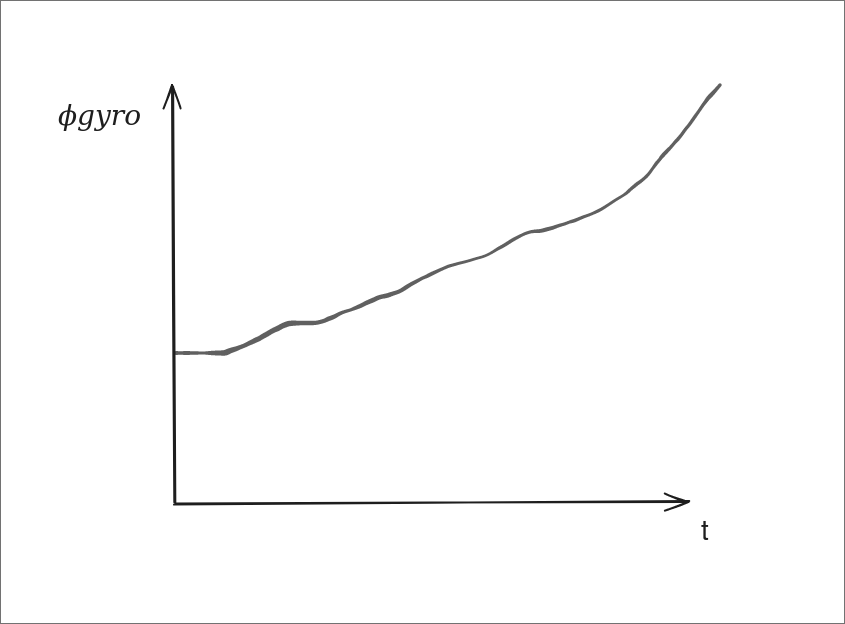
\includegraphics[width=0.7\linewidth]{Figures/drift.png}
	\caption[Dérive du gyroscope]{Dérive du gyroscope.}
\end{figure}


\paragraph{Illustration des limitations des deux capteurs :}
\paragraph*{}
\begin{figure}[!htpb]
	\centering
	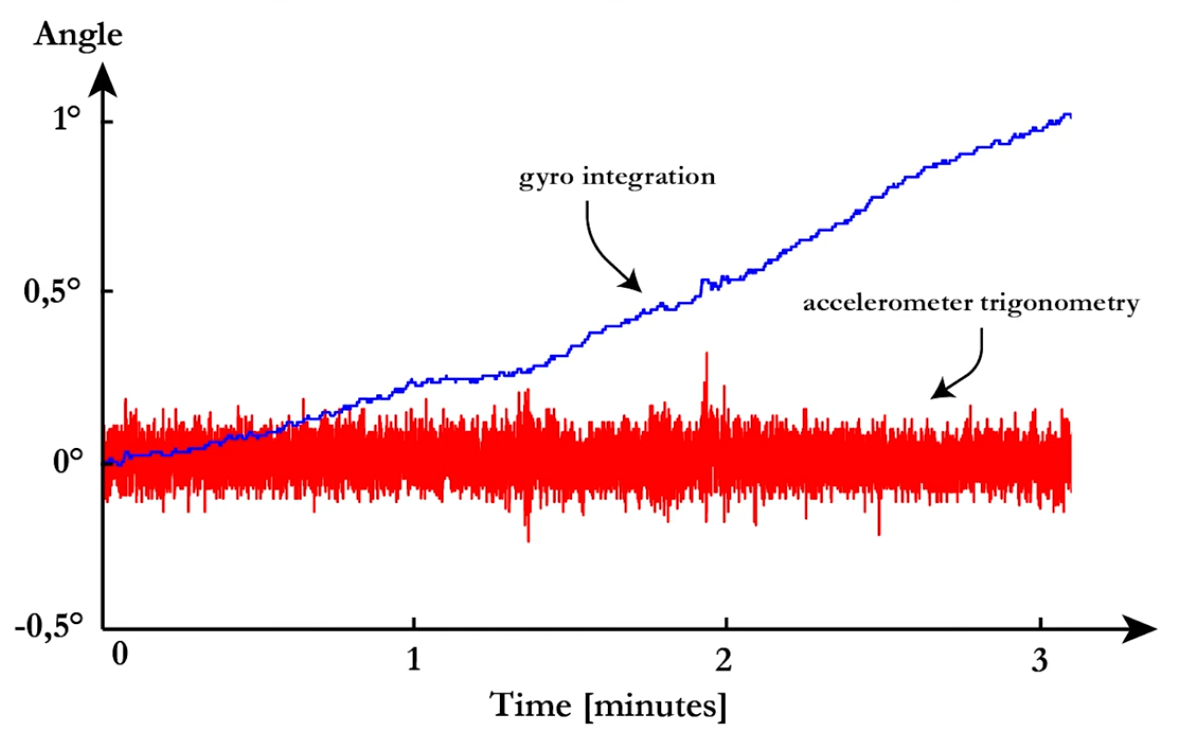
\includegraphics[width=0.7\linewidth]{Figures/accel-gyro-limitations.png}
	\caption{Gyroscope and Accelerometer Limitations.}
\end{figure}


\subsection{Estimation de l'orientation}

\paragraph{Dans la derniere partie, on a vu que le calcule de l'orientation n'est pas exacte et susceptible à des erreurs et des bruits. Pour obtenir une estimation plus précise de l'orientation de l'objet, on doit envisager un estimateur robuste.}

\subsubsection{Filtre Complémentaire (Sensor Fusion)}

\paragraph{Le filtre complémentaire est une méthode courante qui combine des données de capteurs différents pour obtenir une estimation plus précise de l'orientation de l'objet.}
\paragraph*{}
\begin{figure}[!htpb]
	\centering
	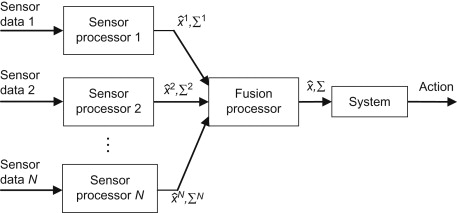
\includegraphics[width=\linewidth]{Figures/sensor-fusion.jpg}
	\caption{Filtre Complémentaire.}
\end{figure}

\paragraph{Donc on peut combiner les deux estimations de l'angle de tangage à partir de l'accéléromètre et du gyroscope en utilisant un filtre complémentaire pour obtenir une estimation plus précise de l'orientation de l'objet.}

\begin{itemize}
	\item \textbf{Le gyroscope :} fonctionne mieux avec un filtrage passe-haut sur l'angle $\phi$ pour remedier aux erreurs cumulées de l'intégration.
	\item \textbf{L'accéléromètre :} est plus efficace lorsqu'un filtre passe-bas élimine les vibrations et autres effets de haute fréquence sur l'angle $\phi$.
\end{itemize}

$\hat{\phi}$ = filtre-passe-haut$(\phi_{gyro})$ + filtre-passe-bas$(\phi_{accel})$


\paragraph{Equations canoniques filtres de premier ordre :}

\begin{itemize}
	\item Filtre Passe Bas : \begin{equation}
		H_{PB}(s) = \frac{1}{1 + \tau s} = \frac{\omega_c}{s + \omega_c}
	\end{equation}
	\item Filtre Passe Haut : \begin{equation}
		H_{PH}(s) = \frac{\tau s}{1 + \tau s} = \frac{s}{s + \omega_c}
	\end{equation}
\end{itemize}

\paragraph{En fusionnant les deux estimations, chaqu'une avec son filtre, on obtient une estimation plus précise de l'orientation de l'objet. qu'on peut schématiser par :}
\paragraph*{}

\begin{figure}[!htpb]
	\centering
	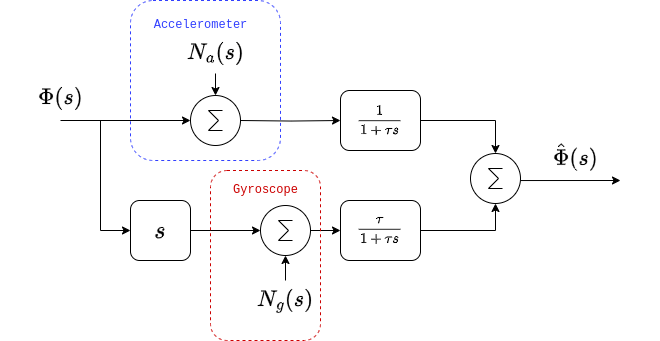
\includegraphics[width=\linewidth]{Figures/pitch-estimation.png}
	\caption{Estimateur de l'orientation.}
\end{figure}

\paragraph{La branche du gyroscope doit se comporter comme un filtre passe-haut et sachant que le gyroscope est de nature derivateur (il donne la derive de l'angle de tangage) on termine la fonction du transfert du filtre passe-haut par un filtre passe-bas de gain $\tau$ ce qui justifie la fonction de Transfert suivante :}

\begin{equation}
	\frac{\tau}{1 + \tau s} = \frac{1}{s} * \frac{\tau s}{1 + \tau s}
\end{equation}

\paragraph{L'equation de l'estimateur de l'angle de tangage devient :}

\begin{equation}
	\hat{\Phi}(s) = \Phi(s) + N_g(s) * \frac{\tau}{1 + \tau s} + N_a(s) * \frac{1}{1 + \tau s}
\end{equation}

\paragraph{On remarque qu'on peut remedier aux bruits $N_a$, $N_g$ de l'accéléromètre et du gyroscope respectivement.}

\subsubsection{Discrétisation des filtres par bloquer d'ordre 1}

\begin{equation}
	H(z) = (1 - z^{-1}) * TZ(TL^{-1}(\frac{H(s)}{s}))
\end{equation}

\begin{itemize}
	\item $H_1(s) = \frac{1}{1 + \tau s} = \frac{\omega_c}{\omega_c + s}$ : \begin{equation}
		H_1(z) = (1 - z^{-1}) * TZ(TL^{-1}(\frac{\omega_c}{s(\omega_c + s)}))
	\end{equation}
	\begin{equation}
		H_1(z) = (1 - z^{-1}) * TZ(TL^{-1}(\frac{1}{s} - \frac{1}{s + \omega_c}))
	\end{equation}
\end{itemize}

\paragraph{On prend $Z(s) = \frac{1}{s} - \frac{1}{s + \omega_c}$}

\paragraph{Transformée de la place inverse :}

\begin{equation}
	TL^{-1}(Z(s)) = z(t) = (1 - e^{-\omega_c t}) * u(t)
\end{equation}

\paragraph{Discretisation de periode d'echantillonnage $T_e = \frac{1}{f_e}$ :}

\begin{equation}
	z(n) = (1 - \alpha^{n}) * u(n)
\end{equation}

\paragraph{Avec $\alpha = e^{-\omega_c T_e}$}

\begin{equation}
	TZ(TL^{-1}(\frac{H_1(s)}{s})) = TZ(z(n)) = \frac{1}{1 - z^{-1}} - \frac{1}{1 - \alpha * z^{-1}}
\end{equation}

\begin{equation}
	H_1(z) = (1 - z^{-1}) * (\frac{1}{1 - z^{-1}} - \frac{1}{1 - \alpha * z^{-1}})
\end{equation}

\begin{equation}
	H_1(z) = \frac{1 - \alpha}{z - \alpha}
\end{equation}

\paragraph{De meme pour $H_2(s)$ on aura la meme forme multipliee par $\tau = \frac{1}{\omega_c}$}

\begin{itemize}
	\item $H_2(s) = \tau \frac{1}{1 + \tau s}$ : \begin{equation}
		H_2(z) = \tau * \frac{1 - \alpha}{z - \alpha}
	\end{equation}
\end{itemize}

\paragraph{Developpement de l'equation de l'estimateur de l'angle de tangage :}

\begin{equation}
	\hat{\Phi}(z) = H_2(z) * \omega_{gyro} + H_1(z) * \Phi_{accel}
\end{equation}

\begin{equation}
	\hat{\Phi}(z) = \tau * \frac{1 - \alpha}{z - \alpha} * \omega_{gyro} + \frac{1 - \alpha}{z - \alpha} * \Phi_{accel}
\end{equation}

\paragraph{Avec $\tau = \frac{\alpha * T_e}{1 - \alpha}$ on aura : $\tau * (1 - \alpha) = \alpha * T_e$}

\paragraph{On peut deduire l'equation de l'estimateur de l'angle de tangage en fonction des mesures de l'accéléromètre et du gyroscope.}

\begin{equation}
	\hat{\Phi}(z) * (z - \alpha) = \alpha * T_e * \omega_{gyro} + (1 - \alpha) * \Phi_{accel}
\end{equation}

\paragraph{En faisant la transformée inverse de Z on obtient :}

\begin{equation}
	\hat{\Phi}(n + 1) - \alpha * \hat{\Phi}(n) = \alpha * T_e * \omega_{gyro} + (1 - \alpha) * \Phi_{accel}
\end{equation}

\begin{equation}
	\hat{\Phi}(n + 1) = \alpha * (\hat{\Phi}(n) + \omega_{gyro} * T_e) + (1 - \alpha) * \Phi_{accel}
\end{equation}

\paragraph{On peut deduire l'equation de l'estimateur de l'angle de tangage en fonction des mesures de l'accéléromètre et du gyroscope.}

\begin{equation}
	\hat{\Phi}(n) = \alpha * (\hat{\Phi}(n - 1) + \omega_{gyro} * T_e) + (1 - \alpha) * \Phi_{accel}
\end{equation}

\section{Schéma final du système}

\paragraph{Le schéma final du système de stabilisation de la barre rotative est composé de trois parties principales :}

\begin{itemize}
	\item \textbf{Correcteur PID $C(s)$ :} \begin{equation}
		C(s) = K_p + \frac{K_i}{s} + K_d * s
	\end{equation}
	\item \textbf{FTBO du système $G(s)$ :} \begin{equation}
		G(s) = \frac{1}{J_\Delta * s^2 + f * s}
	\end{equation}
	\item \textbf{Estimateur d'orientation $\hat{\Phi}(s)$ :} \begin{equation}
		\hat{\Phi}(s) = \frac{\Phi(s) + N_a(s)}{1 + \tau s} + \frac{\tau (s\Phi(s) + N_g(s))}{1 + \tau s}
	\end{equation}
\end{itemize}

\paragraph{Le schéma final du système est illustré par :}
\paragraph*{}
\begin{figure}[!htpb]
	\centering
	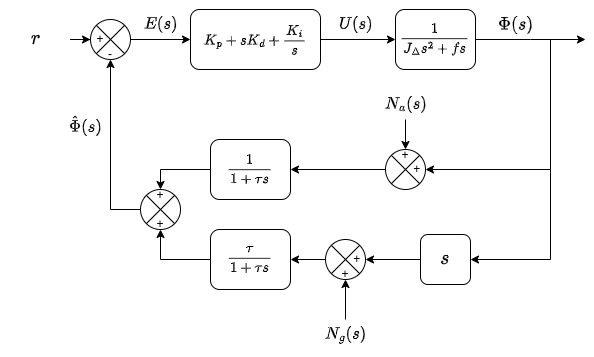
\includegraphics[width=\linewidth]{Figures/final-diagram.png}
	\caption{Schéma final du système.}
\end{figure}

\newpage

\section{Calibration des Capteurs}

\paragraph{Apres avoir remedier aux erreurs et bruits des capteurs, les seuls parametres des modeles des capteurs restants sont les biais des capteurs.}

\paragraph{Pratiquement on mesure en repos un nomber $N$ de mesures (N = 500) pour chaque capteur et on calcule la moyenne des mesures pour chaque axe. Cette methode est efficace en court terme mais en long terme les biais des capteurs peuvent changer.}

\subsection{Biais de l'Accéléromètre}

\paragraph{Pour calibrer le biais de l'accéléromètre, on peut utiliser la mesure de l'accélération gravitationnelle lorsque l'objet est au repos.}

\begin{equation}
	\vec{a} = -R * \vec{g} + b_a(t)
\end{equation}


\begin{equation}
	R = \begin{bmatrix}
		\cos(\phi) \cos(\psi) & \cos(\phi) \sin(\psi) & -\sin(\phi) \\
		\sin(\theta) \sin(\phi) \cos(\psi) - \cos(\theta) \sin(\psi) & \sin(\theta) \sin(\phi) \sin(\psi) + \cos(\theta) \cos(\psi) & \sin(\theta) \cos(\phi) \\
		\cos(\theta) \sin(\phi) \cos(\psi) + \sin(\theta) \sin(\psi) & \cos(\theta) \sin(\phi) \sin(\psi) - \sin(\theta) \cos(\psi) & \cos(\theta) \cos(\phi)
	\end{bmatrix}
\end{equation}

\paragraph{Calibration en repos $\Longrightarrow  \phi = 0$ et $\theta = 0$ et $\psi = 0$}
\paragraph{Donc la matrice de rotation devient :}
\begin{equation}
	R = \begin{bmatrix}
		1 & 0 & 0 \\
		0 & 1 & 0 \\
		0 & 0 & 1
	\end{bmatrix} = I_\mathbb{R^3}
\end{equation}

\begin{equation}
	\vec{b_a} = \begin{bmatrix}
		a_x \\
		a_y \\
		a_z + 9.81
	\end{bmatrix}
\end{equation}


\paragraph{On peut deduire les biais de l'accéléromètre en utilisant les equations suivantes :}

\begin{align}
	b_{ax} &= a_x \\
	b_{ay} &= a_y \\
	b_{az} &= a_z + 9.81
\end{align}

\paragraph{Pour une plage de mesure de l'accéléromètre de $\pm 4g$ on a : g = 8192 (raw sensor)}

\begin{align}
	b_{ax} &= a_x \\
	b_{ay} &= a_y \\
	b_{az} &= a_z + 8192
\end{align}


\subsection{Biais du Gyroscope}

\paragraph{Pour calibrer le biais du gyroscope, on peut utiliser la mesure de la vitesse angulaire lorsque l'objet est au repos.}

\begin{equation}
	\omega = \frac{d\phi}{dt} + b_g(t)
\end{equation}

\begin{equation}
	\omega = 0 + b_g(t)
\end{equation}

\paragraph{On peut deduire le biais du gyroscope en utilisant l'equation suivante :}

\begin{equation}
	\vec{b_g} = \begin{bmatrix}
		\omega_x \\
		\omega_y \\
		\omega_z
	\end{bmatrix}
\end{equation}

\begin{align}
	b_{gx} &= \omega_x \\
	b_{gy} &= \omega_y \\
	b_{gz} &= \omega_z
\end{align}

\section{Conclusion}

\paragraph{Ce qu'il faut envisager au pratique et implementation du système :}

\begin{enumerate}
	\item \textbf{Calibration des capteurs :} Dans un premier temps en fonction setup() on doit calibrer les capteurs pour obtenir les valeurs des biais des capteurs.
	\item \textbf{Estimateur :} Implementation et execution en boucle de l'estimateur d'orientation dimensionné dans la partie précédente avec valeur de $\tau$, $\alpha$ ou bien $f_c$ adaptées.
	\item \textbf{Commande :} Implementation et execution en boucle du correcteur PID pour stabiliser le système.
\end{enumerate}
